% Options for packages loaded elsewhere
\PassOptionsToPackage{unicode}{hyperref}
\PassOptionsToPackage{hyphens}{url}
%
\documentclass[
  12pt,
]{article}
\usepackage{lmodern}
\usepackage{amsmath}
\usepackage{ifxetex,ifluatex}
\ifnum 0\ifxetex 1\fi\ifluatex 1\fi=0 % if pdftex
  \usepackage[T1]{fontenc}
  \usepackage[utf8]{inputenc}
  \usepackage{textcomp} % provide euro and other symbols
  \usepackage{amssymb}
\else % if luatex or xetex
  \usepackage{unicode-math}
  \defaultfontfeatures{Scale=MatchLowercase}
  \defaultfontfeatures[\rmfamily]{Ligatures=TeX,Scale=1}
  \setmainfont[]{Times New Roman}
\fi
% Use upquote if available, for straight quotes in verbatim environments
\IfFileExists{upquote.sty}{\usepackage{upquote}}{}
\IfFileExists{microtype.sty}{% use microtype if available
  \usepackage[]{microtype}
  \UseMicrotypeSet[protrusion]{basicmath} % disable protrusion for tt fonts
}{}
\makeatletter
\@ifundefined{KOMAClassName}{% if non-KOMA class
  \IfFileExists{parskip.sty}{%
    \usepackage{parskip}
  }{% else
    \setlength{\parindent}{0pt}
    \setlength{\parskip}{6pt plus 2pt minus 1pt}}
}{% if KOMA class
  \KOMAoptions{parskip=half}}
\makeatother
\usepackage{xcolor}
\IfFileExists{xurl.sty}{\usepackage{xurl}}{} % add URL line breaks if available
\IfFileExists{bookmark.sty}{\usepackage{bookmark}}{\usepackage{hyperref}}
\hypersetup{
  pdftitle={What's the Catch? Recreational Fishing Trends in North Carolina (1990-2019)},
  pdfauthor={Ardath Dixon, Annie Harshbarger, Eva May},
  hidelinks,
  pdfcreator={LaTeX via pandoc}}
\urlstyle{same} % disable monospaced font for URLs
\usepackage[margin=2.54cm]{geometry}
\usepackage{graphicx}
\makeatletter
\def\maxwidth{\ifdim\Gin@nat@width>\linewidth\linewidth\else\Gin@nat@width\fi}
\def\maxheight{\ifdim\Gin@nat@height>\textheight\textheight\else\Gin@nat@height\fi}
\makeatother
% Scale images if necessary, so that they will not overflow the page
% margins by default, and it is still possible to overwrite the defaults
% using explicit options in \includegraphics[width, height, ...]{}
\setkeys{Gin}{width=\maxwidth,height=\maxheight,keepaspectratio}
% Set default figure placement to htbp
\makeatletter
\def\fps@figure{htbp}
\makeatother
\setlength{\emergencystretch}{3em} % prevent overfull lines
\providecommand{\tightlist}{%
  \setlength{\itemsep}{0pt}\setlength{\parskip}{0pt}}
\setcounter{secnumdepth}{5}
\ifluatex
  \usepackage{selnolig}  % disable illegal ligatures
\fi

\title{What's the Catch? Recreational Fishing Trends in North Carolina
(1990-2019)}
\usepackage{etoolbox}
\makeatletter
\providecommand{\subtitle}[1]{% add subtitle to \maketitle
  \apptocmd{\@title}{\par {\large #1 \par}}{}{}
}
\makeatother
\subtitle{\url{https://github.com/ardathdixon/Data_FinalProject}}
\author{Ardath Dixon, Annie Harshbarger, Eva May}
\date{Spring 2021}

\begin{document}
\maketitle

\newpage
\tableofcontents 
\newpage
\listoftables 
\newpage
\listoffigures 
\newpage

\hypertarget{rationale-and-research-questions}{%
\section{Rationale and Research
Questions}\label{rationale-and-research-questions}}

\begin{itemize}
\item
  Are there trends in the amount of these fish caught over time?
\item
  Do these trends differ for bluefish, black sea bass, and all species
  combined?
\item
  What could these trends look like in the future?
\end{itemize}

\newpage

\hypertarget{dataset-information}{%
\section{Dataset Information}\label{dataset-information}}

Data retrieved from NOAA Marine Recreational Information Program
download query tool

\begin{itemize}
\item
  Bimonthly recreational fisheries catch totals for NC, 1990-2019
\item
  All species, bluefish (\emph{Pomatomus saltatrix}), and black sea bass
  (\emph{Centropristis striata})
\item
  Multiple areas and modes of fishing
\end{itemize}

\newpage

\hypertarget{exploratory-analysis}{%
\section{Exploratory Analysis}\label{exploratory-analysis}}

\begin{verbatim}
## # A tibble: 6 x 8
##    YEAR  WAVE SUB_REG    ST    SP_CODE MODE_FX AREA_X TOT_CAT
##   <dbl> <dbl>   <dbl> <dbl>      <dbl>   <dbl>  <dbl>   <dbl>
## 1  1990     1       6    37 8710010201       3      1 203578.
## 2  1990     1       6    37 8713040113       3      1   9693.
## 3  1990     1       6    37 8713040115       3      1   3987.
## 4  1990     1       6    37 8777020101       7      5 153212.
## 5  1990     1       6    37 8835440102       7      1  82510.
## 6  1990     1       6    37 8835440601       7      1  25388.
\end{verbatim}

\begin{verbatim}
##         DATE TOT_CAT_ALL
## 1 1990-01-01    484714.5
## 2 1990-03-01   2485857.2
## 3 1990-05-01   9215674.2
## 4 1990-07-01  13992342.3
## 5 1990-09-01  11808541.6
## 6 1990-11-01  10354163.5
\end{verbatim}

\newpage

\hypertarget{analysis}{%
\section{Analysis}\label{analysis}}

\begin{verbatim}
## `geom_smooth()` using formula 'y ~ x'
## `geom_smooth()` using formula 'y ~ x'
## `geom_smooth()` using formula 'y ~ x'
\end{verbatim}

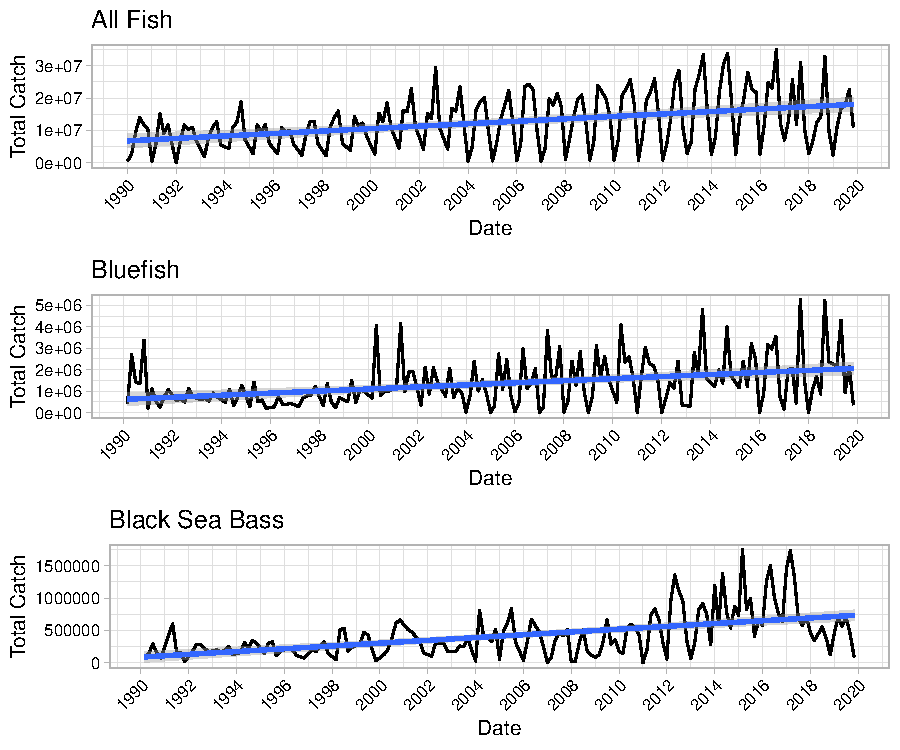
\includegraphics{Report_FishTrends_files/figure-latex/ggplot-1.pdf}

\hypertarget{question-1-are-there-trends-in-the-amount-of-these-fish-caught-over-time}{%
\subsection{Question 1: Are there trends in the amount of these fish
caught over
time?}\label{question-1-are-there-trends-in-the-amount-of-these-fish-caught-over-time}}

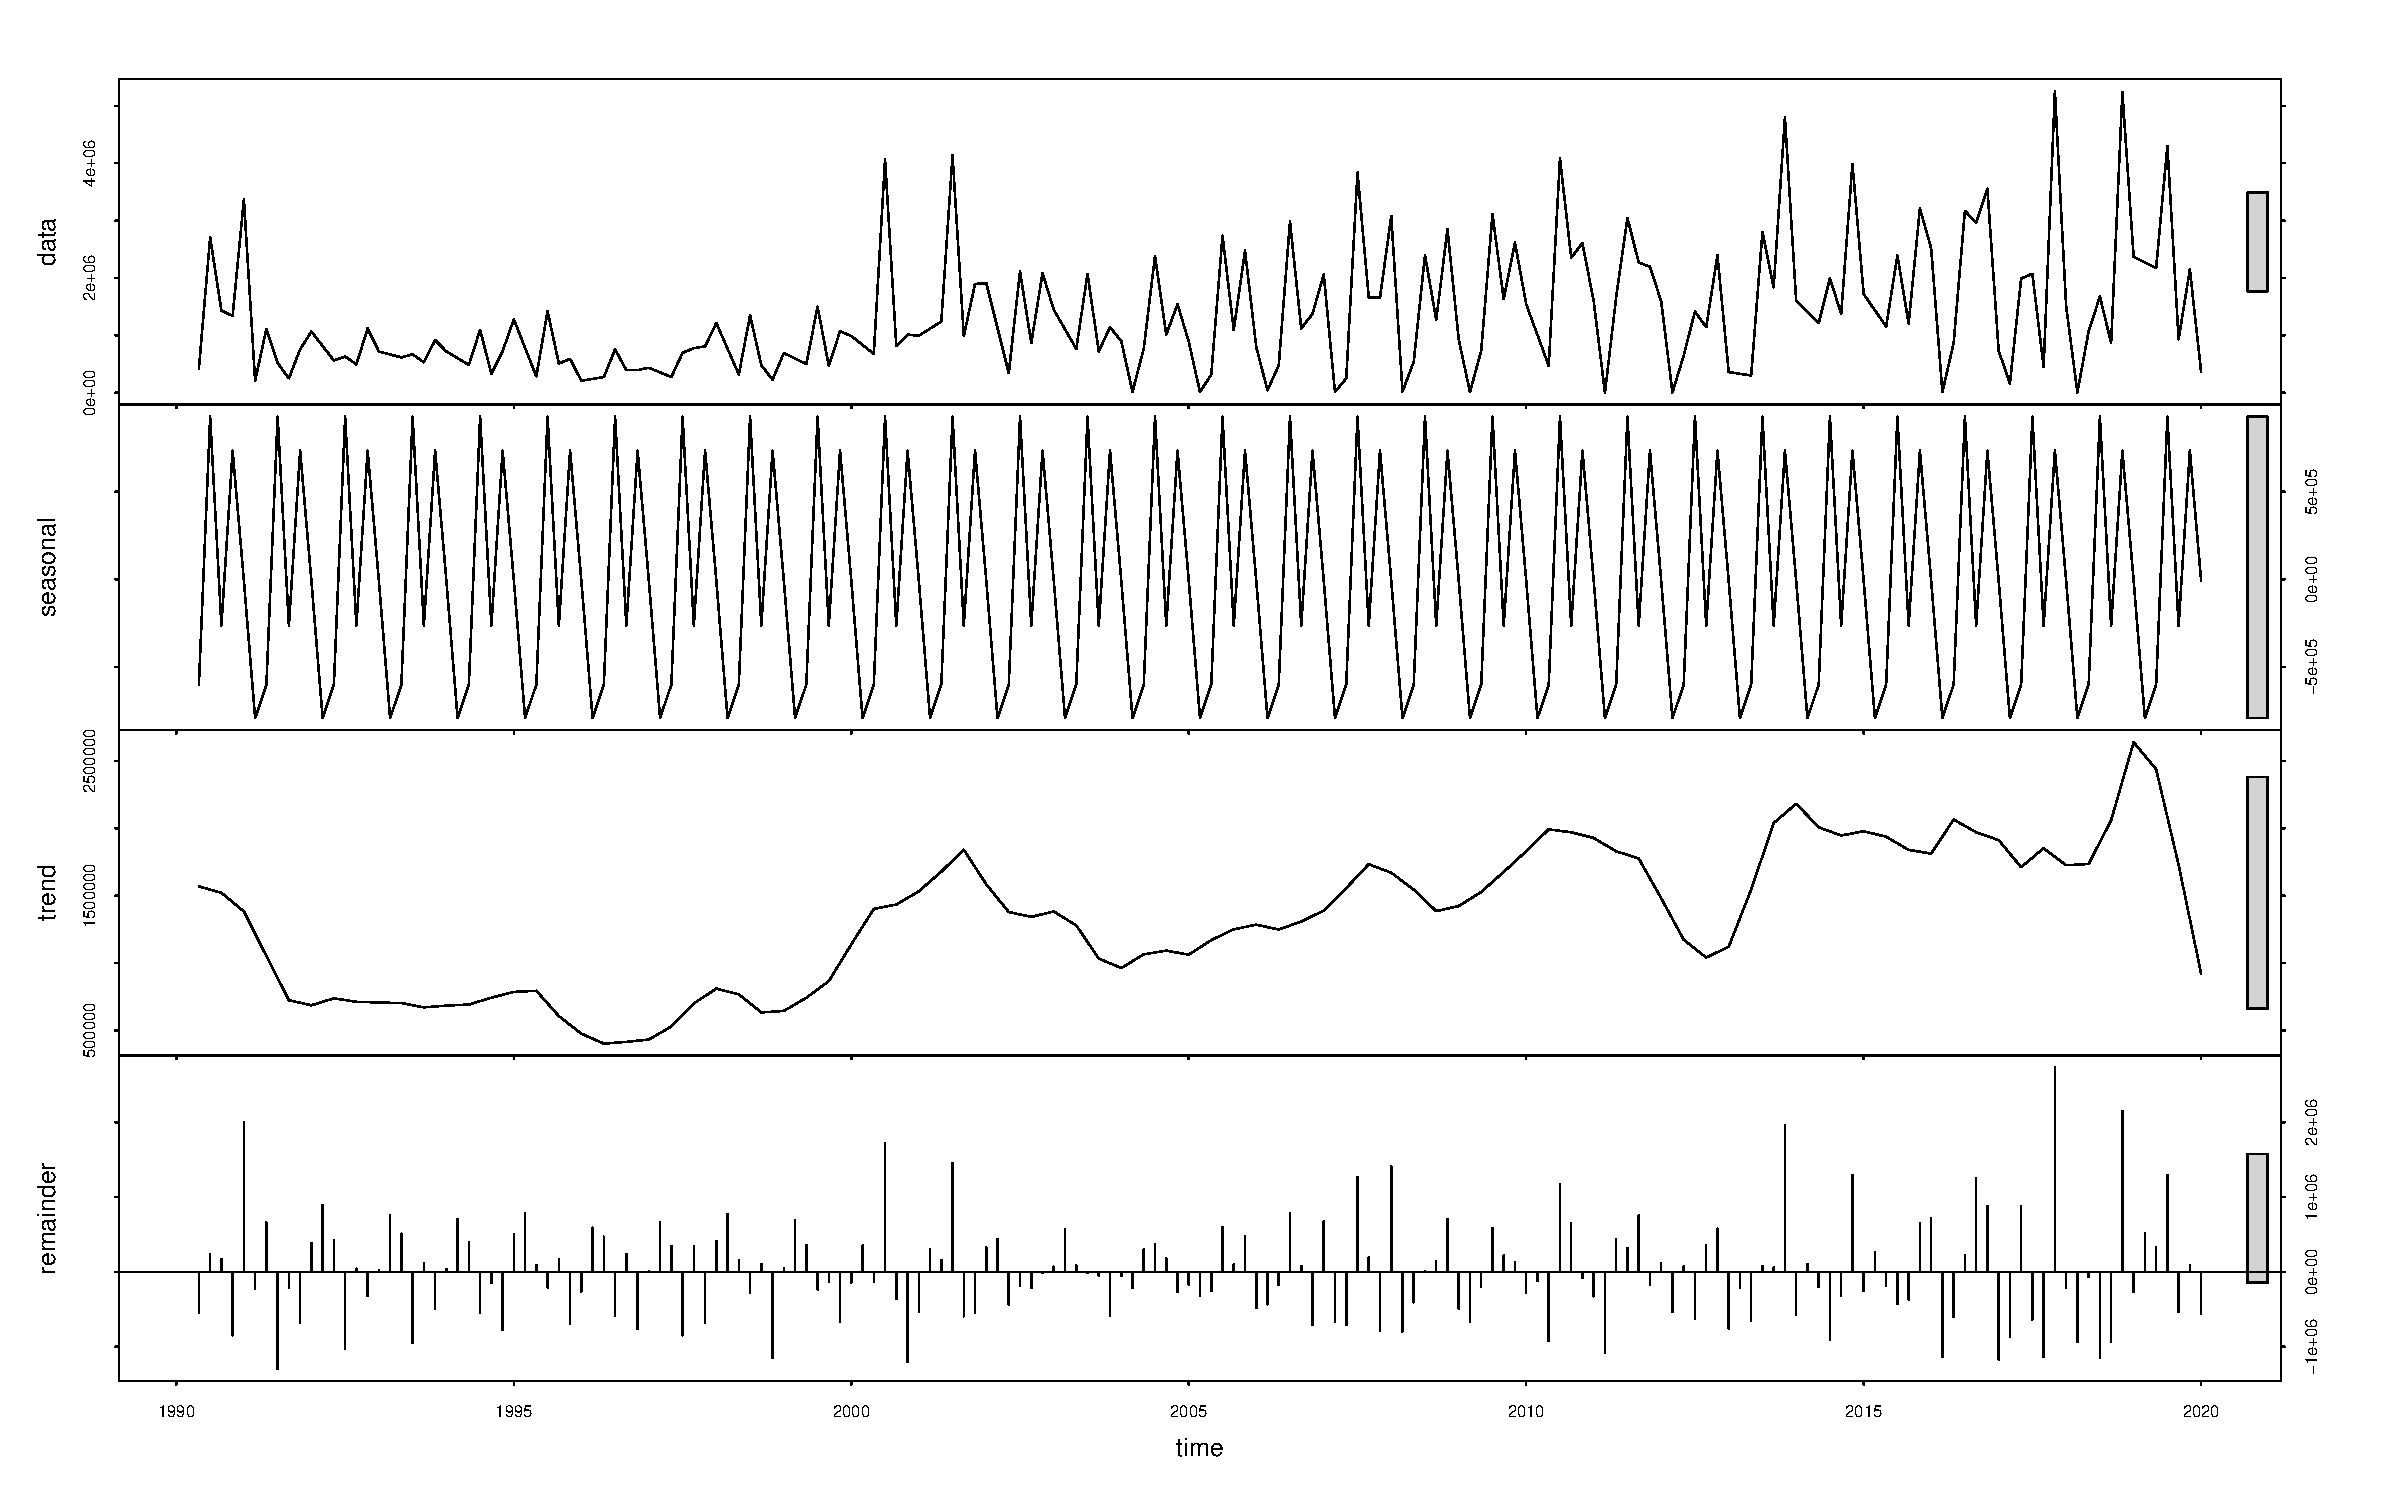
\includegraphics{Report_FishTrends_files/figure-latex/unnamed-chunk-3-1.pdf}

\begin{verbatim}
## tau = 0.49, 2-sided pvalue =< 2.22e-16
\end{verbatim}

\hypertarget{question-2-do-these-trends-differ-for-bluefish-black-sea-bass-and-all-species-combined}{%
\subsection{Question 2: Do these trends differ for bluefish, black sea
bass, and all species
combined?}\label{question-2-do-these-trends-differ-for-bluefish-black-sea-bass-and-all-species-combined}}

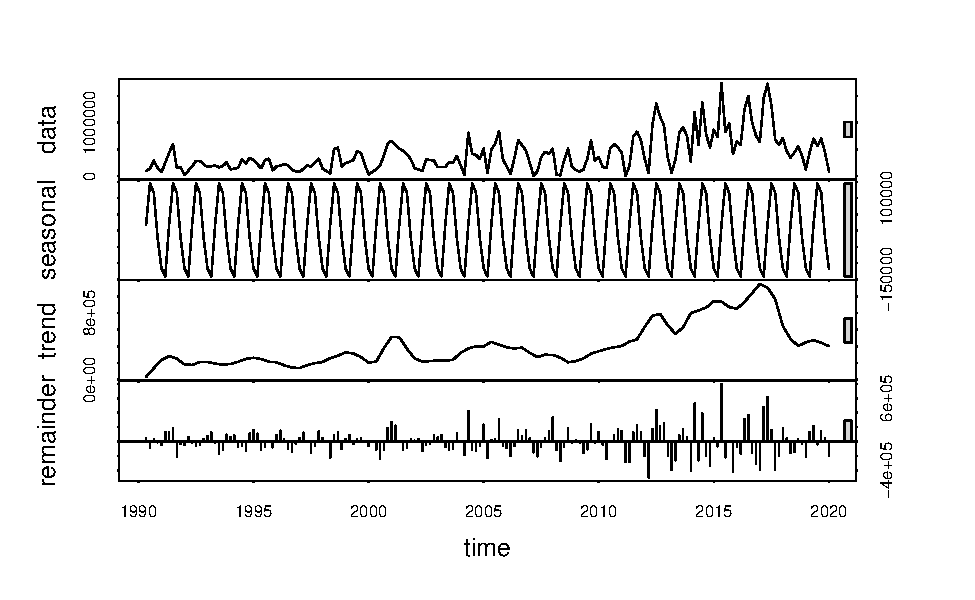
\includegraphics{Report_FishTrends_files/figure-latex/unnamed-chunk-5-1.pdf}

\begin{verbatim}
## tau = 0.324, 2-sided pvalue =8.7489e-10
\end{verbatim}

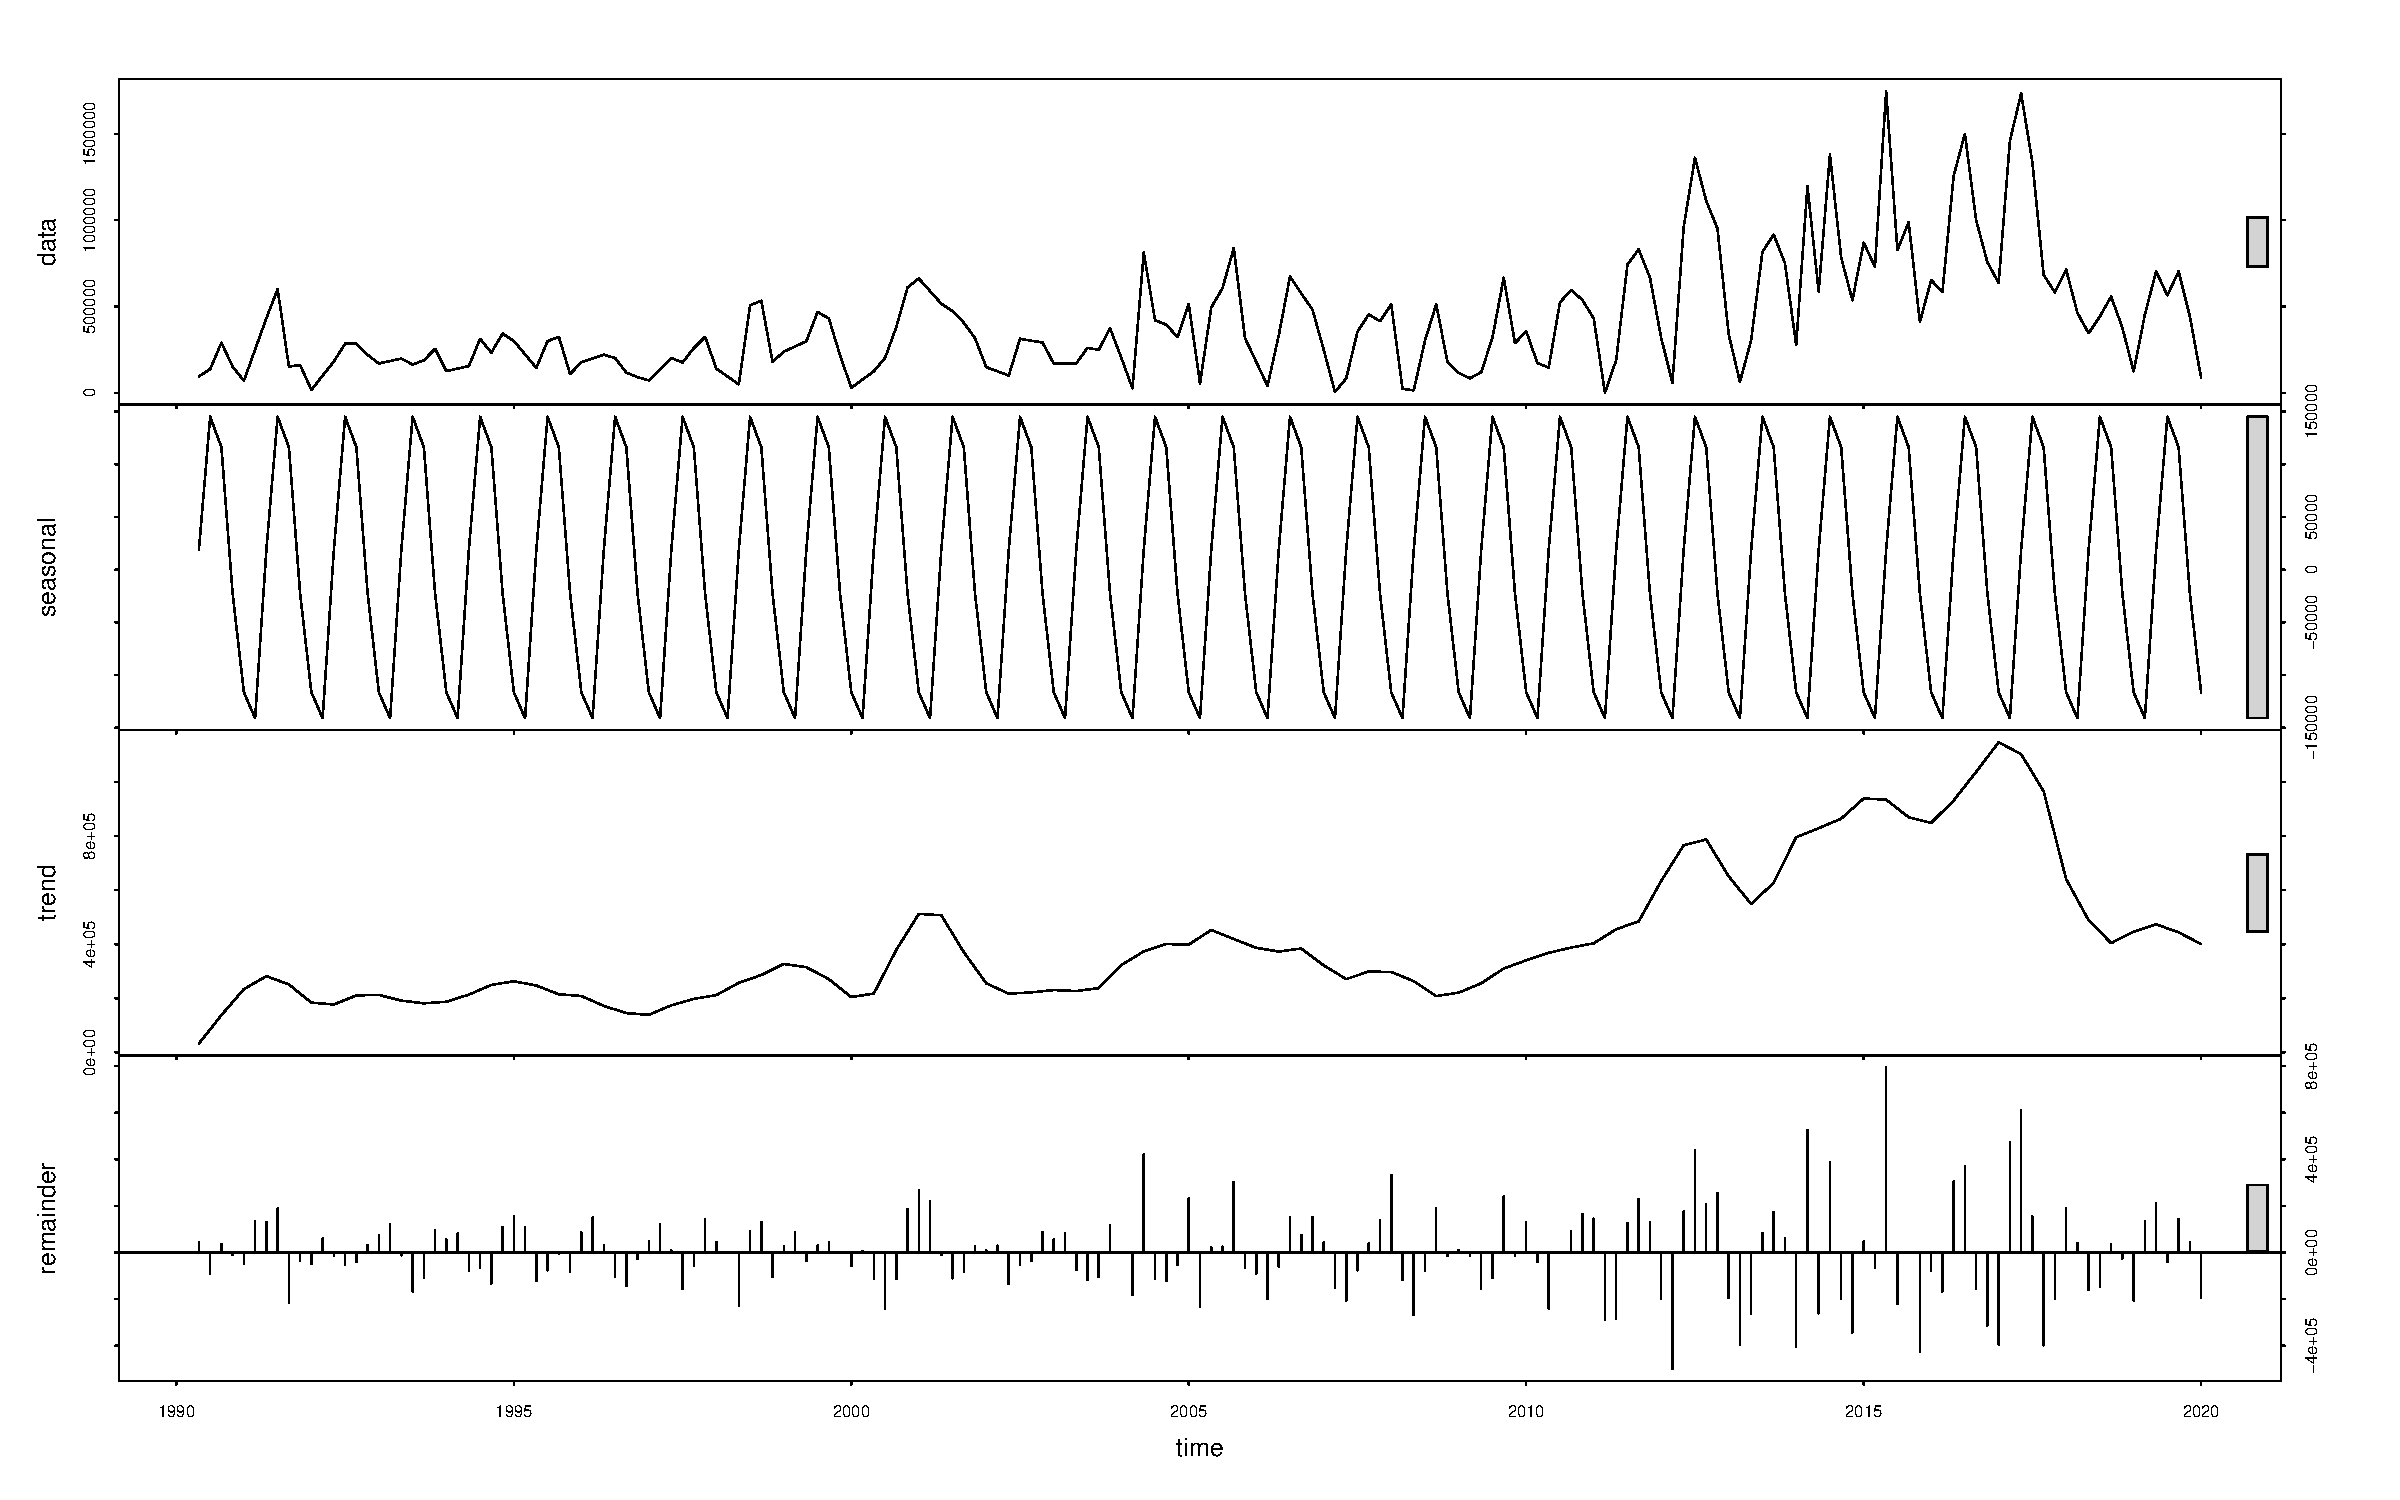
\includegraphics{Report_FishTrends_files/figure-latex/unnamed-chunk-7-1.pdf}

\begin{verbatim}
## tau = 0.41, 2-sided pvalue =8.4377e-15
\end{verbatim}

For both individual species and all species combined, \textbf{reject the
null hypothesis} that there is no trend.

\hypertarget{question-3-what-could-these-trends-look-like-in-the-future}{%
\subsection{Question 3: What could these trends look like in the
future?}\label{question-3-what-could-these-trends-look-like-in-the-future}}

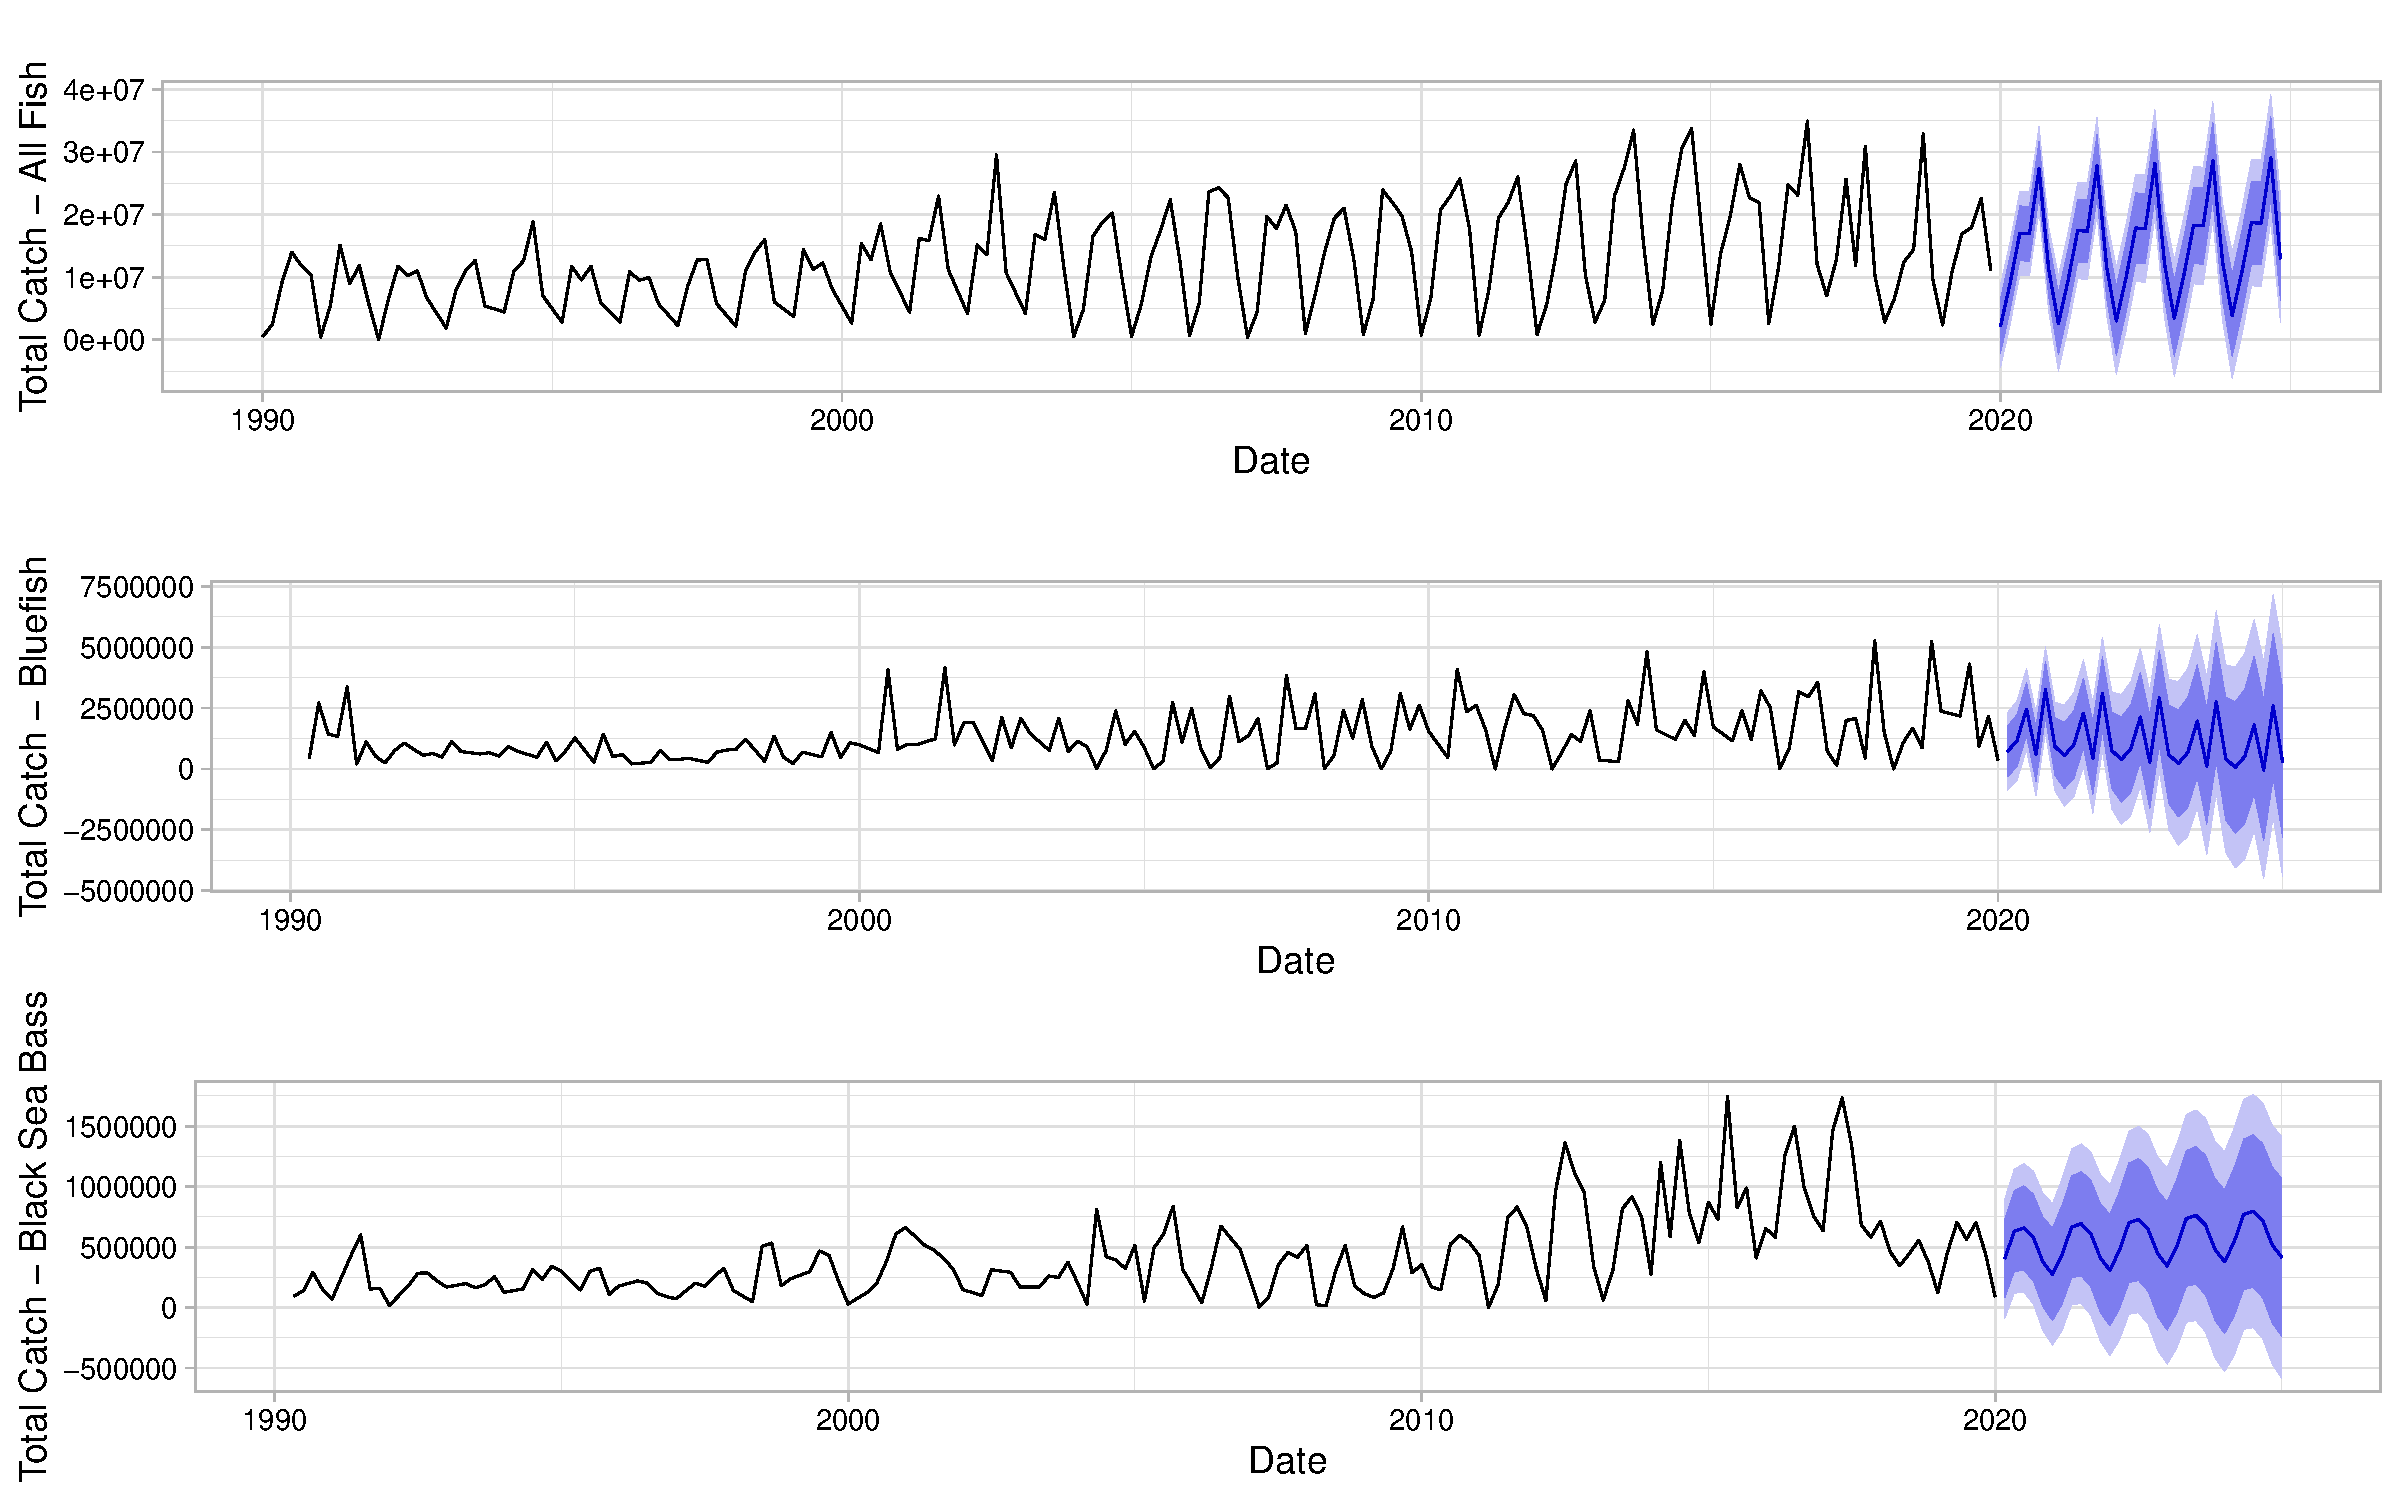
\includegraphics{Report_FishTrends_files/figure-latex/unnamed-chunk-9-1.pdf}

\newpage

\hypertarget{summary-and-conclusions}{%
\section{Summary and Conclusions}\label{summary-and-conclusions}}

\hypertarget{strong-seasonal-trends}{%
\subsection{Strong seasonal trends}\label{strong-seasonal-trends}}

\begin{itemize}
\tightlist
\item
  Bimodal peaks for bluefish
\item
  Possibly due to effort, fish abundance
\end{itemize}

\hypertarget{overall-positive-trend}{%
\subsection{Overall positive trend}\label{overall-positive-trend}}

\begin{itemize}
\tightlist
\item
  Increase in recreational fishing
\item
  Variation from changing regulations, behavior
\end{itemize}

\hypertarget{limitations}{%
\subsection{Limitations}\label{limitations}}

\begin{itemize}
\tightlist
\item
  Data collection: Estimates based on surveys of fishers
\item
  Interpolation
\item
  Uncertainty in forecasting
\end{itemize}

\hypertarget{future-recommendations}{%
\subsection{Future recommendations}\label{future-recommendations}}

\begin{itemize}
\tightlist
\item
  Comparisons of other species or other states
\item
  Catch per unit effort
\item
  Include earlier data
\end{itemize}

\newpage

\hypertarget{references}{%
\section{References}\label{references}}

\textless add references here if relevant, otherwise delete this
section\textgreater{}

\end{document}
